%% abtex2-modelo-relatorio-tecnico.tex, v-1.7.1 laurocesar
%% Copyright 2012-2013 by abnTeX2 group at http://abntex2.googlecode.com/ 
%%
%% This work may be distributed and/or modified under the
%% conditions of the LaTeX Project Public License, either version 1.3
%% of this license or (at your option) any later version.
%% The latest version of this license is in
%%   http://www.latex-project.org/lppl.txt
%% and version 1.3 or later is part of all distributions of LaTeX
%% version 2005/12/01 or later.
%%
%% This work has the LPPL maintenance status `maintained'.
%% 
%% The Current Maintainer of this work is the abnTeX2 team, led
%% by Lauro César Araujo. Further information are available on 
%% http://abntex2.googlecode.com/
%%
%% This work consists of the files abntex2-modelo-relatorio-tecnico.tex,
%% abntex2-modelo-include-comandos and abntex2-modelo-references.bib
%%

% ------------------------------------------------------------------------
% ------------------------------------------------------------------------
% abnTeX2: Modelo de Relatório Técnico/Acadêmico em conformidade com 
% ABNT NBR 10719:2011 Informação e documentação - Relatório técnico e/ou
% científico - Apresentação
% ------------------------------------------------------------------------ 
% ------------------------------------------------------------------------

\documentclass[
	% -- opções da classe memoir --
	12pt,				% tamanho da fonte
	openright,			% capítulos começam em pág ímpar (insere página vazia caso preciso)
	oneside,			% para impressão em verso e anverso. Oposto a oneside
	a4paper,			% tamanho do papel. 
	% -- opções da classe abntex2 --
	chapter=TITLE,		% títulos de capítulos convertidos em letras maiúsculas
	%section=TITLE,		% títulos de seções convertidos em letras maiúsculas
	%subsection=TITLE,	% títulos de subseções convertidos em letras maiúsculas
	%subsubsection=TITLE,% títulos de subsubseções convertidos em letras maiúsculas
	% -- opções do pacote babel --
	english,			% idioma adicional para hifenização
	french,				% idioma adicional para hifenização
	spanish,			% idioma adicional para hifenização
	brazil,				% o último idioma é o principal do documento
	]{abntex2}


% ---
% PACOTES
% ---

% ---
% Pacotes fundamentais 
% ---
\usepackage{cmap}				% Mapear caracteres especiais no PDF
\usepackage{lmodern}			% Usa a fonte Latin Modern
\usepackage[T1]{fontenc}		% Selecao de codigos de fonte.
\usepackage[utf8]{inputenc}		% Codificacao do documento (conversão automática dos acentos)
\usepackage{indentfirst}		% Indenta o primeiro parágrafo de cada seção.
\usepackage{color}				% Controle das cores
\usepackage{graphicx}			% Inclusão de gráficos
\graphicspath{ {img/} }
\usepackage{caption}
\usepackage{float}
\usepackage[most]{tcolorbox}

\captionsetup{
  font=footnotesize,
  justification=raggedright,
  singlelinecheck=false
}
 
% ---

% ---
% Pacotes adicionais, usados no anexo do modelo de folha de identificação
% ---
\usepackage{multicol}
\usepackage{multirow}
% ---
	
% ---
% Pacotes adicionais, usados apenas no âmbito do Modelo Canônico do abnteX2
% ---
\usepackage{lipsum}				% para geração de dummy text
% ---

% ---
% Pacotes de citações
% ---
\usepackage[brazilian,hyperpageref]{backref}	 % Paginas com as citações na bibl
\usepackage[alf]{abntex2cite}	% Citações padrão ABNT

% --- 
% CONFIGURAÇÕES DE PACOTES
% --- 

% ---
% Configurações do pacote backref
% Usado sem a opção hyperpageref de backref
\renewcommand{\backrefpagesname}{Citado na(s) página(s):~}
% Texto padrão antes do número das páginas
\renewcommand{\backref}{}
% Define os textos da citação
\renewcommand*{\backrefalt}[4]{
	\ifcase #1 %
		Nenhuma citação no texto.%
	\or
		Citado na página #2.%
	\else
		Citado #1 vezes nas páginas #2.%
	\fi}%
% ---

% ---
% Informações de dados para CAPA e FOLHA DE ROSTO
% ---
\titulo{Relatório Final de Projeto\\ Ysto\\ Automação Residencial}

\autor{Fabiano da Rosa Gomes}
\local{Porto Alegre}
\data{2017}
\instituicao{
  Serviço Nacional de Aprendizagem Comercial do Rio Grande do Sul\\ Faculdade Senac Porto Alegre\\ Curso Superior de Tecnologia em Análise e Desenvolvimento de Sistemas}
\tipotrabalho{Relatório final de projeto}
% O preambulo deve conter o tipo do trabalho, o objetivo, 
% o nome da instituição e a área de concentração 
\preambulo{Relatório Final de Projeto, apresentado como requisito parcial à obtenção do grau de Técnologo em Análise e Desenvolvimento de Sistemas, pela Faculdade Senac Porto Alegre.
Orientador: Prof. Me. Luciano Zanuz.}
% ---

% ---
% Configurações de aparência do PDF final

% alterando o aspecto da cor azul
\definecolor{blue}{RGB}{41,5,195}

% informações do PDF
\makeatletter
\hypersetup{
     	%pagebackref=true,
		pdftitle={\@title}, 
		pdfauthor={\@author},
    	pdfsubject={\imprimirpreambulo},
	    pdfcreator={LaTeX with abnTeX2},
		pdfkeywords={abnt}{latex}{abntex}{abntex2}{relatório técnico}, 
		colorlinks=true,       		% false: boxed links; true: colored links
    	linkcolor=black,          	% color of internal links
    	citecolor=black,        		% color of links to bibliography
    	filecolor=magenta,      		% color of file links
		urlcolor=black,
		bookmarksdepth=4
}
\makeatother
% --- 

% --- 
% Espaçamentos entre linhas e parágrafos 
% --- 

\usepackage{tabularx}

% O tamanho do parágrafo é dado por:
\setlength{\parindent}{1.3cm}

% Controle do espaçamento entre um parágrafo e outro:
\setlength{\parskip}{0.2cm}  % tente também \onelineskip

% ---
% compila o indice
% ---
\makeindex
% ---

% ----
% Início do documento
% ----
\begin{document}

% Retira espaço extra obsoleto entre as frases.
\frenchspacing 

% ----------------------------------------------------------
% ELEMENTOS PRÉ-TEXTUAIS
% ----------------------------------------------------------
% \pretextual

% ---
% Capa
% ---
\imprimircapa
% ---

% ---
% Folha de rosto
% (o * indica que haverá a ficha bibliográfica)
% ---
\imprimirfolhaderosto*
% ---

% ---
% RESUMO
% ---

% resumo na língua vernácula (obrigatório)
\begin{resumo}
O presente projeto propõem um sistema de automação residencial, provendo o controle e o acionamento de dispositivos que são alimentados por energia elétrica em corrente alternada, disponível nas tomadas residenciais. Para tanto, usa um conjunto composto de uma placa ESP8266 (wifi) e uma RaspberryPI (central de controle). Nesta central de controle é possível manipular mais de um módulo wifi, ligando e desligando suas saídas através do protocolo MQTT. Foi utilizado as linguagens de programação C, Python e Javascript no desenvolvimento deste projeto.

 \vspace{\onelineskip}
    
 \noindent
 \textbf{Palavras-chaves}: automação residencial. iot. mqtt. python. javascript.
\end{resumo}
% ---

% ---
% inserir lista de ilustrações
% ---
\pdfbookmark[0]{\listfigurename}{lof}
\listoffigures*
\cleardoublepage
% ---

% ---
% inserir lista de tabelas
% ---
\pdfbookmark[0]{\listtablename}{lot}
\listoftables*
\cleardoublepage
% ---

% ---
% inserir lista de abreviaturas e siglas
% ---
\begin{siglas}
  \item[AC] Alternate Current
  \item[API] Application Program Interface
  \item[AURESIDE] Associação Brasileira de Automação Residencial e Predial
  \item[CHPD] Chip Select
  \item [CORS] Cross-Origin Resource Sharing
  \item[CRUD] Acrônimo do inglês para Create, Read, Update e Delete
  \item[ER] Entidade Relacionamento
  \item[GND] Ground
  \item[GPIO] General Purpose Input/Output
  \item[IBGE] Instituto Brasileiro de Geografia e Estatística
  \item[IDE] Integrated Development Environment
  \item[IHM] Interface Homem Máquina
  \item[JSON] JavaScript Object Notation
  \item[M2M] Machine to Machine
  \item[MA] Módulo Auxiliar
  \item[MD5] Message-Digest algorithm 5
  \item[MQTT] Message Queue Telemetry Transport
  \item[MVR] Model-View-Router
  \item[NPM] Node Package Manager
  \item[ORM] Object-relational mapping
  \item[PSP] Personal Software Process
  \item[PWA] Progressive Web Apps
  \item[REST] REpresentational State Transfer
  \item[RST] Reset
  \item[RX] Receiver
  \item[SOC] System-On-Chip
  \item[TX] Transmitter
  \item[VCC] Power Supply
  \item[W3C] World Wide Web Consortium
\end{siglas}

% ---

% ---
% inserir o sumario
% ---
\pdfbookmark[0]{\contentsname}{toc}
\tableofcontents*
\cleardoublepage
% ---


% ----------------------------------------------------------
% ELEMENTOS TEXTUAIS
% ----------------------------------------------------------
\textual

% ----------------------------------------------------------
% Capitulo com exemplos de comandos inseridos de arquivo externo 
% ----------------------------------------------------------

\include{abntex2-modelo-include-comandos}

% ---
% Capitulos
% ---
\chapter{Apresentação geral do projeto}

A quantidade de produtos eletroeletrônicos cresce cada vez mais nas residências brasileiras, conforme mostra a pesquisa realizada pelo Instituto Brasileiro de Geografia e Estatística (IBGE) em 2016. A tabela \ref{ibge} apresenta a presença em números percentuais de alguns eletrodomésticos nos lares brasileiros.

\begin{table}[H]
   \caption{Presença dos produtos eletroeletrônicos nos domicílios brasileiros}
   \label{ibge}
{
   \begin{tabular}{lllll}
   \toprule
   Produto & 2012 & 2013 & 2014 & 2015 \\
   \midrule \midrule
   
    Fogões & 98,75\% & 98,76\% & 98,81\% & 98,84\% \\
    Televisores & 97,20\% & 97,16\% & 97,14\% & 97,14\% \\
    Refrigeradores & 96,65\% & 97,21\% & 97,56\% & 97,83\% \\
    Rádio & 80,86\% & 75,71\% & 72,08\% & 69,23\% \\
    Máquinas de lavar & 55,14\% & 57,46\% & 58,68\% & 61,14\% \\
    Freezer & 16,66\% & 17,05\% & 16,48\% & 16,88\% \\
   
   \bottomrule
   \end{tabular}
}{
   \legend{Fonte: IBGE 2016}
}
\end{table}

Junto com o crescimento de produtos deste segmento, o acesso à internet também cresceu muito nos últimos anos. Em matéria do portal G1 de 06 de Abril de 2016\footnote{http://g1.globo.com/tecnologia/noticia/2016/04/internet-chega-pela-1-vez-mais-de-50-das-casas-nobrasil-mostra-ibge.html acessado em 14/11/2017}, é destaque a quantidade de casas com acesso a internet, 50 por cento em média. Estes números acabam fortalecendo um outro mercado que nasce quase como uma consequência do consumo de eletrônicos e acesso a internet, o mercado de automação residencial.
Automação residencial, ou domótica, segundo o Departamento de Informática (DIN) da Universidade Estadual de Maringá (UEM) pode ser definido como:
\begin{citacao}
O termo domótica, é uma fusão da palavra latina domus (casa) e do moderno robótica. A domótica, que também pode ser referenciada por expressões como "smart building", "intelligent building", "edifícios inteligentes", é um novo domínio de aplicação tecnológica, tendo como objetivo básico melhorar a qualidade de vida, reduzindo o trabalho doméstico, aumentando o bem estar e a segurança de seus habitantes e visa também uma utilização racional e planejada dos diversos meios de consumo. A domótica procura uma melhor integração através da automatização nas áreas de segurança, de comunicação e de controle, e gestão de fluídos. \cite{DOMOTICA}
\end{citacao}

Com base nas definições conceituais anteriores, é correto afirmar que a domótica cuida da integração de sistemas e tem por finalidade tornar o ambiente doméstico e os diversos equipamentos que fazem parte dele mais fáceis de serem utilizados por qualquer morador da casa, com ou sem conhecimentos especializados em tecnologia da informação. Investir em automação residencial garante praticidade e objetividade no dia a dia sem prejudicar o conforto e segurança\footnote{http://overbr.com.br/artigos/por-que-investir-em-automacao-residencial acessado em 14/11/2017}. Este mercado oferta diversas possibilidades, como o desenvolvimento de sistemas personalizados para atender necessidades específicas, a busca por redução de consumo energético ou ainda a preocupação com a segurança podem ser a motivação para busca de soluções nesta área. Analisando um mercado maior que o nosso e que normalmente dita as tendências de futuro, a Associação Brasileira de Automação Residencial e Predial (AURESIDE) destaca:

\begin{citacao}
Pesquisas da Parks Associates mostram que mais de 100 milhões de lares dos EUA não tinham um dispositivo doméstico inteligente no final de 2016. Analistas da empresa internacional observam que alcançar essas famílias exige investimentos contínuos para criar experiências únicas e personalizadas para os moradores... 
A empresa de pesquisa, em seu serviço NUMBERS, estima que até 2020,mais de 12 milhões de lares americanos terão um detector inteligente de vazamento de água, mais de 40 milhões terão um termostato inteligente, quase 50 milhões terão uma lâmpada inteligente e cerca de 14 milhões terão um controlador doméstico inteligente. A Conferência CONNECTIONS deste ano examinará as oportunidades de investimento no IOT que impulsionarão esse crescimento e sua adoção em soluções domésticas inteligentes. \cite{MERCADO}.
\end{citacao}

Diante deste cenário promissor, soluções mais acessíveis precisam ser criadas pensando na realidade brasileira. Falar sobre ter uma opção acessível não está ligado somente as questões financeiras, embora estas tenham um peso significativo na escolha. Facilidade de obter os componentes, configurá-los e integrar isso com padrões existentes são o diferencial deste projeto.

Este projeto apresenta uma solução para automação residencial, baseada em padrões abertos que não dependem do pagamento de licensas ou direitos autorais, o que facilita a integração com outros sistemas ou dispositivos. Também utiliza componentes eletrônicos de fácil acesso e com preços razoáveis, levando em conta as soluções existentes de mercado nacional.

\begin{figure}[H]
\caption{\label{domotica} Possibilidades da domótica nos dias de hoje}
\includegraphics[scale=0.20]{img/casa-conectada.png}
\legend{Fonte: Website da Aureside \cite{MERCADO}}
\end{figure}

 A Figura \ref{domotica} mostra, de forma esquemática, as possibilidades disponíveis com um sistema de domótica em nossas residências. Possibilidades estas que vão do controle de acesso a residencia, monitoramento de áreas específicas, controle do ambiente através de sensores de temperatura ou ainda a integração com outros dispositivos inteligentes como um aparelho de TV ou central de multimídia.

\chapter{Definição do problema}

Diariamente novos dispositivos são inseridos no cotidiano da sociedade, essa variedade de "coisas" que fazem parte do cotidiano podem acabar se tornando um problema, principalmente para pessoas com pouca prática na configuração e utilização destes novos e modernos aparelhos. Neste ambiente desconexo, qualquer nova aquisição, como um novo ar condicionado ou uma fechadura eletrônica passam a ser mais um dispositivo com características novas e configurações diferentes que necessitam ser administrados por estes moradores.
As primeiras interfaces homem máquina (IHM) que utilizam o controle remoto, por rádio frequência, normalmente são as opções mais comuns e variadas nas residências atuais. A figura \ref{controle} mostra algumas variações desta interface para controle das coisas de casa.

\begin{figure}[H]
\caption{\label{controle} Exemplos de IHM convencionais}
\includegraphics[scale=0.35]{img/controle-remoto.png}
\legend{Fonte: Website da digitaltrends}
\end{figure}

É comum que todos estes aparelhos funcionem de forma independente e desconectadas, cabendo aos usuários desvendar os segredos de cada IHM. O que deveria trazer facilidade e comodidade pode facilmente se tornar um forte motivo para aquela nova aquisição cair rapidamente em desuso ou simplesmente não ser utilizada da maneira correta. Outro cenário muito comum é a eleição de um "especialista" em novas tecnologias, as vezes um filho ou sobrinho descolado que domina as novidades recém chegadas. O fato é que esse acumulo de possibilidades gera insatisfação e porque não dizer frustração nos usuários que gostariam apenas de desfrutar das soluções e confortos que estes bens prometem trazer e nem sempre cumprem essa tarefa a contento.

Nos últimos anos, uma tendência tem se mostrado forte, a integração destes aparelhos, empresas grandes como Google\footnote{https://madeby.google.com/home/} , Amazon\footnote{https://www.amazon.com/dp/B00X4WHP5E} e Apple\footnote{https://www.apple.com/homepod} tem investido tempo e dinheiro para criar soluções que entregam uma experiência mais integrada ao cotidiano das pessoas. Este processo envolve a adaptação dos aparelhos existentes em conjunto com uma integração a novos sistemas e interfaces mais amigáveis. Todas as soluções citadas anteriormente utilizam o hábito dos moradores para fazer uma mapa e uma agenda de eventos, sugerindo com o passar do tempo certas ações que antes dependiam exclusivamente do controle humano, isso introduz o que convencionou chamar de Aprendizagem de Máquina associado a Sistemas de Recomendações. Estes sistemas prometem ser assistentes pessoais e conforme as demonstrações destes fabricantes, realmente vão mudar a maneira como nos relacionamos com as máquinas.

Neste processo, a captura de hábitos e o aprendizado que estas novas tecnologias prometem conseguir vão levar às próximas gerações a experimentar uma integração com as máquinas muito mais natural e porque não dizer orgânica. Fazer diferente o que de certa forma se acostuma pelo hábito é o que as soluções destas empresas propõem, interfaces de controle por voz, aprendizado de máquina e conexão com serviços externos são algumas das novidades que fazem parte do núcleo desta nova família de aplicativos e dispositivos.

Este mercado aposta em três itens para captar estes novos consumidores:
\begin{itemize}
    \item[a)] Conforto;
    \item[b)] Segurança;
    \item[c)] Integração.
\end{itemize}

Nem sempre a tecnologia costuma ficar disponível para a grande maioria de forma rápida, tornar projetos de eletrônica e informática uma realidade no Brasil muitas vezes é um desafio e isso por vezes nos deixa nos tempos das cavernas em relação a paises desenvolvidos, mesmo no mais otimista dos cenários ainda estamos longe de ter acesso as soluções de domótica existentes no exterior. As principais questões que dificultam o acesso a essas soluções são em primeiro lugar a falta de interesse comercial de trazer isso para nosso país, nossa infraestrutura embora tenha melhorado, ainda está longe do ideal. Os custos de serviço de \textit{telecom} associado as altas taxas de importação de eletrônicos inviabilizam a chegada destas facilidades as lojas do nosso país.
Estas dificuldades não vão fazer com que as pessoas deixem de querer isso e de alguma forma estas necessidades serão sanadas, dentro deste contexto que nasce o projeto de automação residencial chamado Ysto, este projeto se propõem a contemplar os itens acima citados de forma mais simples e a um uma fração do preço dos existentes na atualidade.

Fazer a aquisição de dados, transformá-los em informação útil e decidir o que fazer com esta informação disponibilizando uma interface simples e unificada será o escopo deste projeto, tudo isso a um custo mínimo. A figura \ref{custos} mostra uma estimativa de preço para montagem de uma central de controle e um módulo auxiliar.

\begin{figure}[H]
\caption{\label{custos} Levantamento aproximado de custos}
\includegraphics[scale=0.4]{img/custos.png}
\legend{Fonte: Autor do projeto}
\end{figure}

Estes valores foram coletados em sites como mercado livre e solda fria, são apenas estimativas e médias de preços, ou seja, podem variar. Uma alternativa muito interessante para aquisição dos componentes principais do sistema, a RaspberryPI e o ESP-01 são os sites chineses que disponibilizam estes componentes a preços muito mais atrativos. Apenas como efeito de ilustração, o site Aliexpress vende conjuntos de cinco ESP-01 a R\$32,00 é possível optar por um módulo pronto como o da figura \ref{modulo-ali}.

\begin{figure}[H]
\caption{\label{modulo-ali} Alternativa pronta para o MA}
\includegraphics[scale=0.4]{img/modulo-ali.png}
\legend{Fonte: Website da Aliexpress}
\end{figure}

Este módulo reduziria nosso custo para aproximadamente R\$60.00 e teríamos algo muito prático e de fácil utilização.



\chapter{Objetivos}
Esta seção apresenta os objetivos do trabalho, divididos em objetivo geral e objetivos específicos.

\section{Objetivo geral}

O objetivo geral deste trabalho é desenvolver um sistema que viabilize a automação de atividades em uma casa, a partir de uma interface simples de controle e acionamento de dispositivos, este controle remoto universal é acessado através do celular de qualquer um dos moradores.

\section{Objetivos específicos}
Para atingir o objetivo geral deste projeto, será necessário atingir os seguintes objetivos específicos:

\begin{itemize}
    \item[a)] Implementar um aplicativo que possa ser acessado via smartfone, Android e IOS, para controlar os dispositivos;
    \item[b)] Elaborar um controle de acesso através deste aplicativo para impedir que ações indesejadas ocorram;
    \item[c)] Elaborar uma interface de controle que possa ser conectado a eletrodomésticos comuns permitindo controla-los de forma remota.
\end{itemize}


\chapter{Análise de tecnologias e ferramentas}
No desenvolvimento deste trabalho foram usados as seguintes ferramentas e tecnologias.

\section{RaspberryPI}
O RaspberryPI é um computador com dimensões reduzidas, do tamanho de um cartão de crédito, que disponibiliza diversos IO para integração. Escolhido por oferecer um bom poder de processamento (que impacta no tempo de resposta dos acionamentos), apresentar um baixo custo e de fácil aquisição no mercado local. É a central de controle do projeto, onde ficam hospedados os serviços e os aplicativos deste projeto, a Figura \ref{raspberryPI} mostra uma placa de forma esquemática. \cite{RaspberryPI2017}

\begin{figure}[H]
\caption{\label{raspberryPI}Diagrama esquemático de uma RaspberryPI}
\includegraphics[scale=0.15]{img/raspberrypi.png}
\legend{Fonte: Wikipedia}
\end{figure}

\section{ESP8266}
O ESP8266 é um System-On-Chip (SOC) com WIFI embutido, é produzido pela empresa Espressif, disponibiliza diversos IO e é compatível com o \textit{framework} do Arduíno. (Epressif, 2017). Neste projeto, funciona como um acoplamento a eletrodomésticos existentes, trazendo um interface de comunicação WIFI para dispositivos que não a possuem, é o chamado Módulo Auxiliar (MA), a Figura \ref{esp8266} mostra o modelo 01 desta placa e sua pinagem. \cite{Esp82662017}

\begin{figure}[H]
\caption{\label{esp8266}Diagrama esquemático de uma ESP8266-01}
\includegraphics[scale=0.5]{img/esp8266-01f.png}
\legend{Fonte: Autor do projeto}
\end{figure}

\section{Arduíno}
Segundo definição do site Embarcados:

\begin{citacao}
Arduíno é uma plataforma de código aberto (hardware e software) criada em 2005 pelo italiano Massimo Banzi (e outros colaboradores) para auxiliar no ensino de eletrônica para estudantes de design e artistas. O objetivo principal foi o de criar uma plataforma de baixo custo, para que os estudantes pudessem desenvolver seus protótipos com o menor custo possível. Outro ponto interessante do projeto, foi a proposta de criar uma plataforma de código aberto, disponível para a comunidade o que ajudou em muito no seu desenvolvimento. \cite{OQUEARDUINO}
\end{citacao}

Foi a ferramenta escolhida para o desenvolvimento do \textit{firmware} do Módulo Auxiliar (MA) em função da facilidade de uso e por oferecer um grande número de bibliotecas para os mais diversos hardwares de mercado. \cite{Arduino2017}

\section{Javascript}
Javascript é a principal linguagem de programação para desenvolvimento de aplicativos para browsers de internet. É utilizada para o desenvolvimento da interface com usuário final. 

\section{Python}
Segundo o site do projeto:

\begin{citacao}
Python é uma linguagem de programação de alto nível, interpretada, de script, imperativa, orientada a objetos, funcional, de tipagem dinâmica e forte.  \cite{PYTHON}
\end{citacao}

Foi a alternativa encontrada, quando dos problemas de performance na utilização de NodeJS \cite{NodeJS2017}. Em um período curto de tempo, quatro dias, toda API para controlar os módulos auxiliares foi reescrita.

\section{SQLite}
A wikipedia faz uma tradução do site do projeto, segundo eles:

\begin{citacao}
SQLite é uma biblioteca em linguagem C que implementa um banco de dados SQL embutido. Programas que usam a biblioteca SQLite podem ter acesso a banco de dados SQL sem executar um processo Sistema de Gerenciamento de Banco Dados (SGBD) separado. \cite{SQLITE}
\end{citacao}
Foi a opção escolhida devido a performace e falicidade de implementação para ambientes com Linux embarcado.

\section{MQTT}
MQTT é um protocolo de comunicação do tipo Machine to Machine (M2M) desenvolvido pela IBM no inicio dos anos 2000 como solução de comunicação entre hardwares de baixa capacidade de computação de dados com equipamentos mais robustos. Este protocolo serve de "cola" entre todos os entes de um sistema heterogêneo, onde servidores, computadores pessoais, smartfones e microcontroladores precisam conversar. Neste projeto é utilizado como o meio de comunicação entre todos os MAs e a central de controle. \cite{Mqtt2017}

\section{Mosquitto}
Mosquitto é um Broker, ou central de controle de mensagens, que utiliza o protocolo MQTT para troca de mensagens em dispositivos diversos sobre o protoclo TCP. Está instalado e configurado como serviço na RaspberryPI portanto, fazendo parte da central de controle.\cite{MOSQUITTO}

\section{Debian Linux}
Debian Linux é uma das primeiras distribuições Linux 1993, conhecido por seu rigoroso critério na aprovação de pacotes e na consequente robustez do sistema. Oferece uma licença para uso pessoal ou comercial que não onera o projeto. É o sistema operacional da central de controle. \cite{Debian2017}

\section{Geany IDE}
Segundo o site do projeto, Geany é um editor de textos que usa o kit gráfico GTK+ com características básicas de uma \textit{Integrated Development Environment} (IDE), tradução do autor. Todo o código escrito neste projeto usou esta IDE. \cite{GEANY2017}

\section{Schemacrawler}
Segundo o site do projeto, Schemacrawler é uma ferramenta de descoberta e compreensão de esquemas de banco de dados, tradução do autor. Esta ferramenta foi utilizada para a partir do banco de dados gerado pelo módulo de \textit{Object-relational mapping} (ORM), mapear as tabelas e relacionamentos, traduzindo para um diagrama Entidade Relacionamento. \cite{CRAWLER}

\section{Git SCM}
Segundo o site do projeto, Git é um sistema de controle distribuído de código fonte aberto, projetado para lidar com tudo, de pequenos a grandes projetos com velocidade e eficiência, tradução do autor. Todo material deste projeto incluindo este relatório estão versionados e controlados com o Git. \cite{GIT2017}

\section{Gliffy}
Gliffy é uma extensão do google chrome para criação e edição de diagramas, usada neste projeto para elaboração dos diagramas de BPM e fluxo de dados. \cite{GLIFFY}

\section{VueJS}
Vuejs é um framework \textit{open-source} utilizado para desenvolvimento de interfaces gráficas para ambientes web. Foi escolhido para este projeto devido a simplicidade e facilidade de uso, envolve um \textit{setup} de ambiente de desenvolvimento que requer poucos recursos(é possível iniciar o desenvolvimento sem o uso de NodeJS e sua coleção de ferramentas). Separa o tratamento de dados da visualização destes o que facilita a modularização do projeto. \cite{VUEJS}

\section{Skeleton}
Skeleton é um \textit{template} para desenvolvimento de interfaces web, oferece uma estrutura miníma de html e css. Foi a opções escolhida em função do tamanho reduzido, da simplicidade para iniciar o desenvolvimento e rapidez em obter resultados. \cite{SKELETON}

\chapter{Descrição da solução}

Este projeto possui duas grandes partes, os Módulos Auxiliares (MA) e a central de controle. A figura \ref{dispositivos} mostra um diagrama geral de comunicação de um dispositivo acoplado a um Módulo Auxiliar (MA) com a central de controle.

\begin{figure}[H]
\caption{\label{dispositivos} Topologia da solução}
\includegraphics[scale=0.5]{img/arquitetura-basica-2.png}
\legend{Fonte: Autor do projeto}
\end{figure}

O principal diferencial deste projeto e a API de controle dos dispositivo, esta API segue o padrão RESt de implementação o que permite que qualquer cliente que tenha a capacidade de integrar-se a APIs deste tipo possam fazer uso dela.

\section{Módulos Auxiliares}
Estes módulos são acoplados a eletrodomésticos e são compostos por uma placa ESP8266 modelo ESP-01, todo processo de desenvolvimento do \textit{firmware} até a gravação deste \textit{firrmware} na placa ESP-01 é feito utilizando a IDE do Arduíno. Também são usados bibliotecas do framework Arduíno para comunicação através do protocolo MQTT com a central de controle.

\subsection{Esquema eletrônico do MA}
Foi desenvolvido um circuito para acoplar a placa ESP-01 a um relé, este é responsável por fazer o acionamento de cargas AC (Corrente Alternada, tradução do inglês). A figura \ref{sch-ma} mostra este circuíto de forma esquemática.

\begin{figure}[H]
\caption{\label{sch-ma} Esquemático eletrônico do MA}
\includegraphics[scale=0.25]{img/sch-ma.png}
\legend{Fonte: Autor do projeto}
\end{figure}

\subsection{Programação do \textit{firmware} do MA}
No processo de desenvolvimento do \textit{firmware} do MA foi utilizado a IDE Arduíno, a figura \ref{arduino-ide} mostra com um trecho do firmware de controle do MA.

\begin{figure}[H]
\caption{\label{arduino-ide} Arduíno IDE}
\includegraphics[scale=0.3]{img/ide-arduino.png}
\legend{Fonte: Autor do projeto}
\end{figure}

O processo de gravação do \textit{firmware} na placa ESP-01 utiliza um gravador que é acoplado a uma das portas USB do computador, a figura \ref{gravacao-firmware} mostra como é este gravador e a montagem do módulo para gravação de \textit{firmware}.

\begin{figure}[H]
\caption{\label{gravacao-firmware} Gravação do \textit{firmware} no MA}
\includegraphics[scale=0.11]{img/gravador-firmware.png}
\legend{Fonte: Autor do projeto}
\end{figure}

\section{Central de controle}
A central de controle é um micro computador com dimensões reduzidas, o modelo é uma RaspberryPI tipo B com 512MB de RAM e um cartão de memória do tipo SD card com 8GB de memória disponível. Neste computador estão instalados os seguintes programas:

\begin{itemize}
    \item[a)] Sistema operacional Debian na versão 8;
    \item[b)] Broker MQTT Mosquitto versão 1.4.14;
    \item[c)] NodeJS versão 8.2.1;
    \item[d)] Sqlite3 versão 3.8.7.
\end{itemize}

Na figura \ref{raspberry-case} é possível ver o computador montado em uma caixa de acrílico.

\begin{figure}[H]
\caption{\label{raspberry-case} Central de controle}
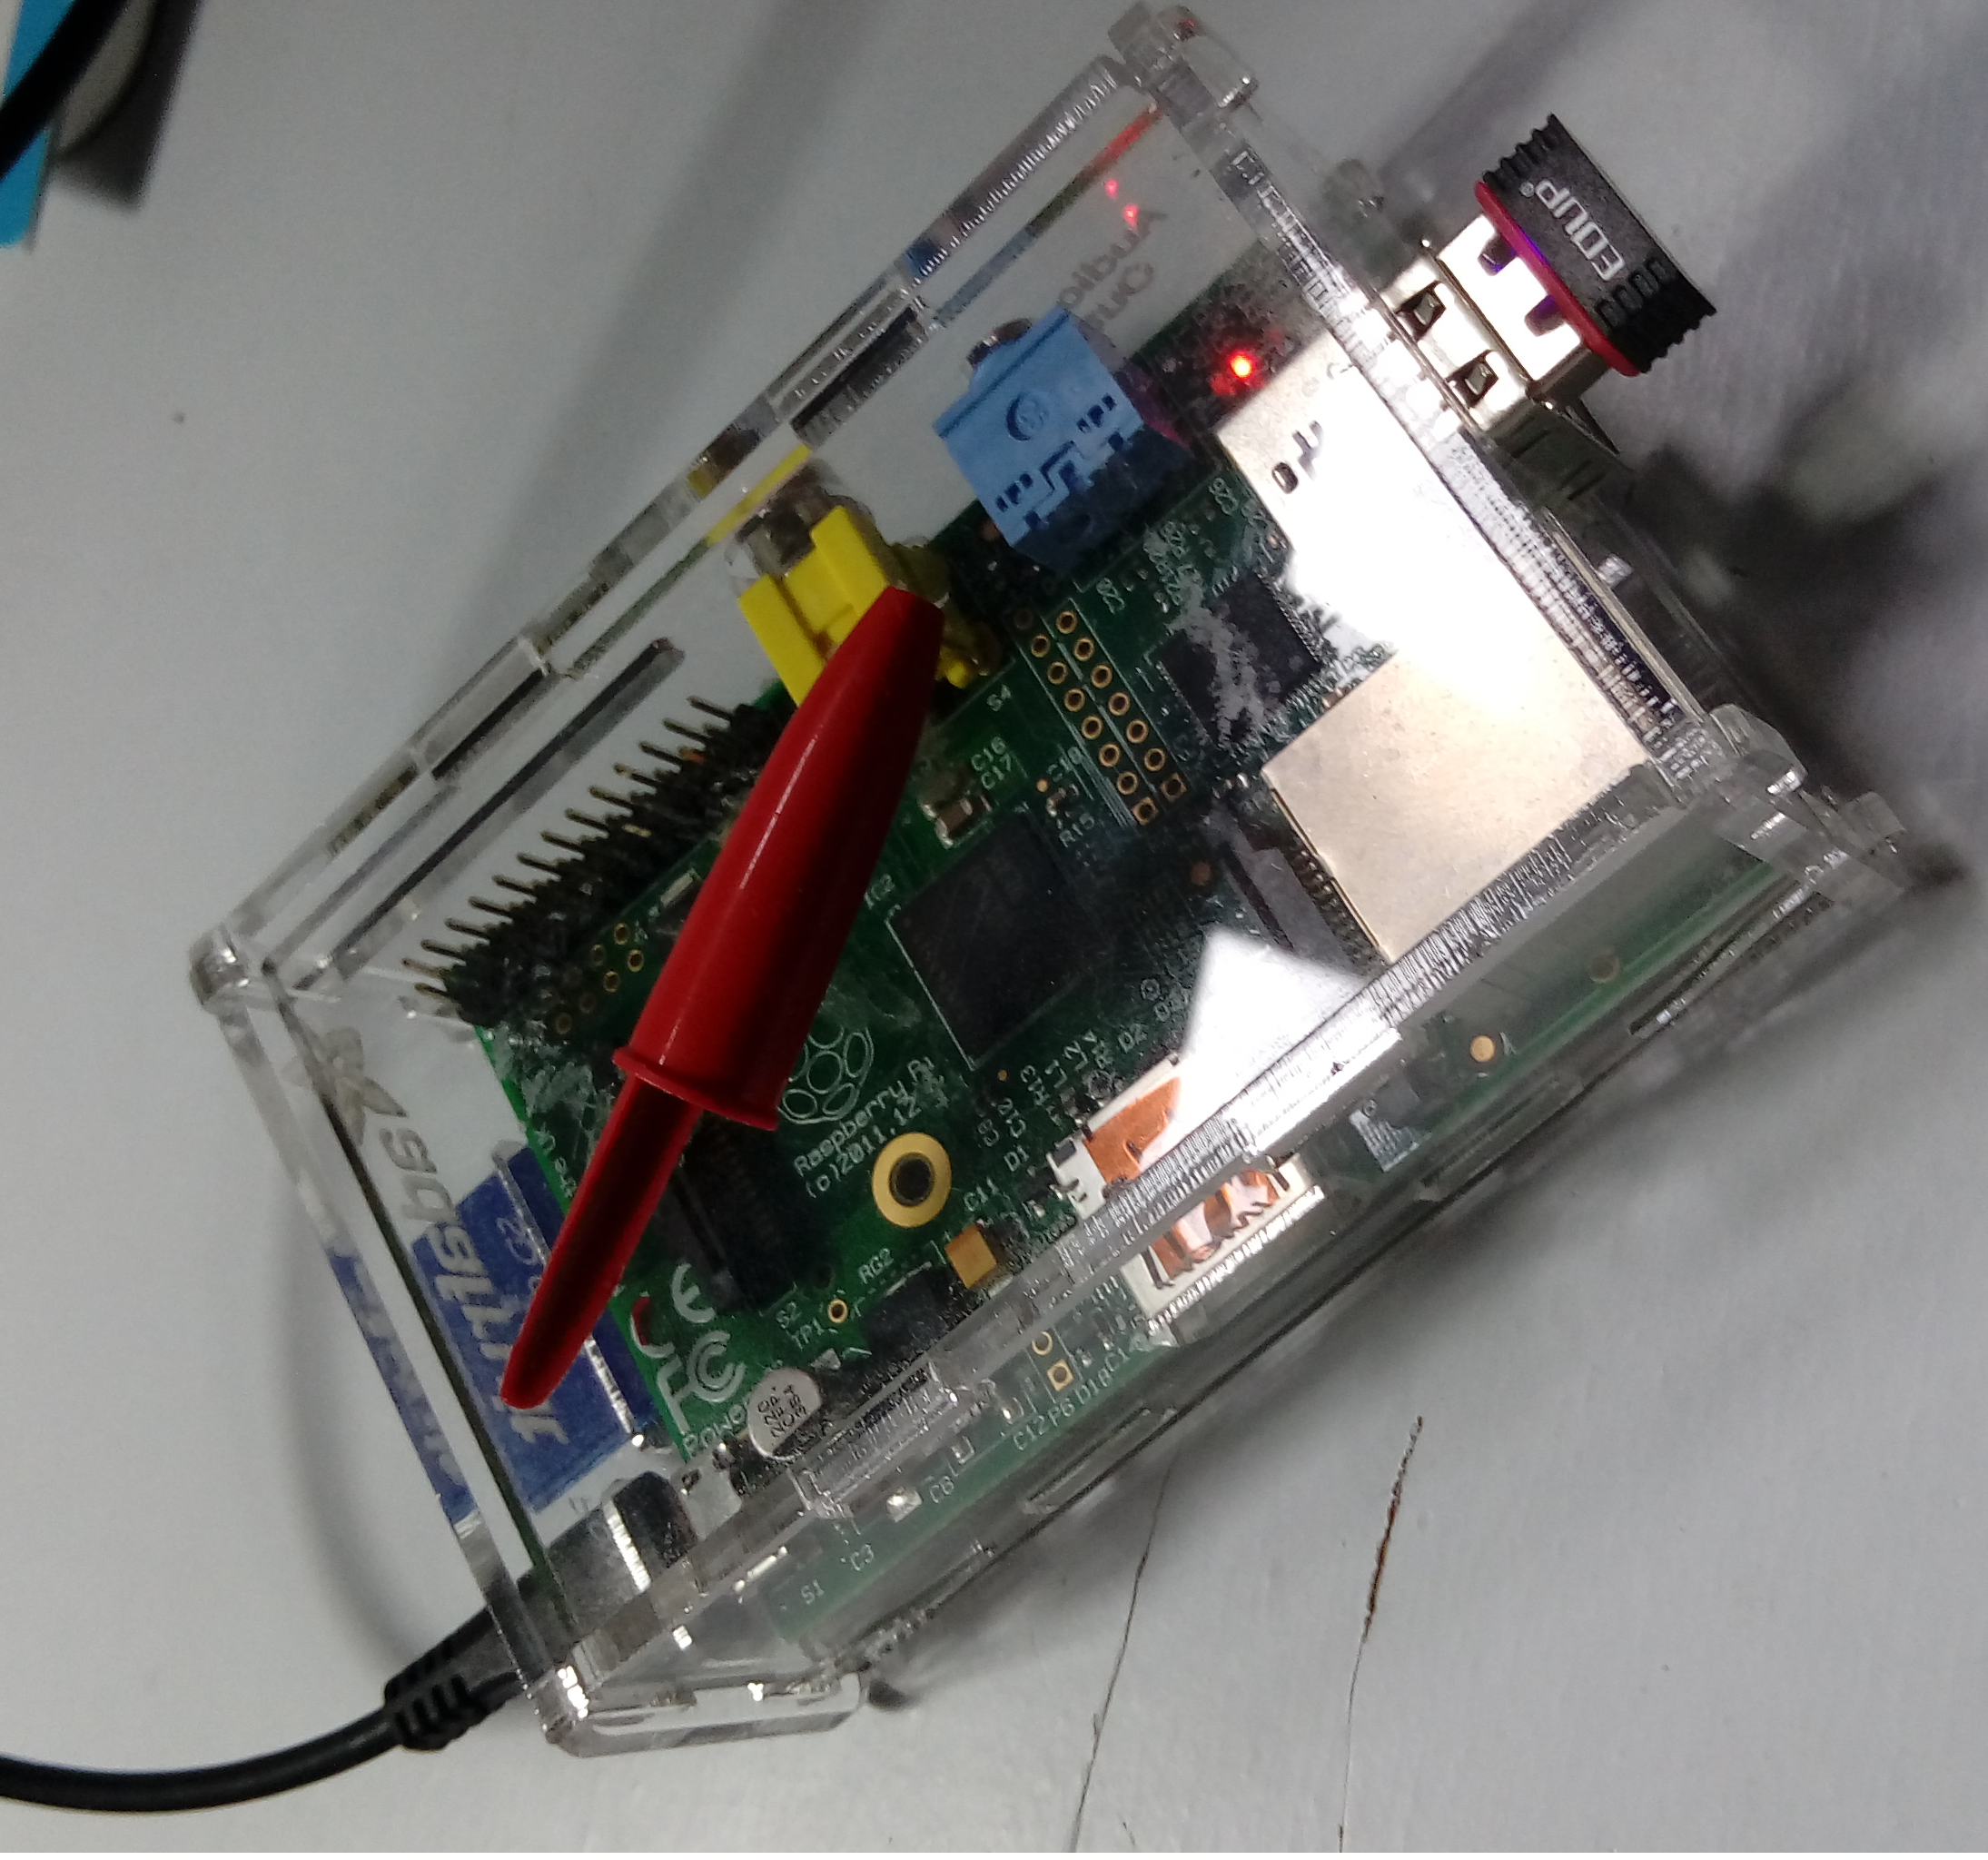
\includegraphics[scale=0.15]{img/rpi.png}
\legend{Fonte: Autor do projeto}
\end{figure}

Na figura \ref{ysto-central} mostra a coleção de serviços e aplicativos que estão hospedados na central de controle.

\begin{figure}[H]
\caption{\label{ysto-central} Esquemático de serviços da central de controle}
\includegraphics[scale=0.5]{img/ysto-diagrama-central.png}
\legend{Fonte: Autor do projeto}
\end{figure}

A troca de mensagens será feita utilizando o protocolo chamado Telemetry Transport Message Queue (MQTT), este protocolo além de possuir um baixo consumo de banda (as mensagens são relativamente pequenas em comparação com outros protocolos que trafegam no mesmo meio, http por exemplo) ainda fornece ferramentas necessárias para:

\begin{itemize}
    \item[a)] Fazer o controle de quem pode trocar mensagens na nossa rede de dispositivos;
    \item[b)] Garantir a entrega das mensagens;
    \item[c)] Integração com aplicativos de mercado em diversas plataformas mobile ou \textit{Desktop}.
\end{itemize}

Este Dashboard será um Appweb do tipo \textit{Mobile First} ou seja, seus layouts serão adaptados para as telas de telefones, tablets e computadores.

\section{Funcionamento do protocolo MQTT}
Este projeto baseia-se fortemente no funcionamento do protocolo MQTT (IBM, 2017), é importante entender como este funciona pois tem reflexo direto em como este projeto opera. Este protocolo de comunicação permite estabelecer uma maneira simples de comunicação entre múltiplos dispositivos, podendo:

\begin{itemize}
    \item[a)] Enviar um comando para uma saída;
    \item[b)] Ler uma entrada e publicar os dados lidos.
\end{itemize}

A figura \ref{mqtt-1} exemplifica o funcionamento do envio de um comando para uma saída do sistema.

\begin{figure}[H]
\caption{\label{mqtt-1} Mensagem sendo enviada via MQTT}
\includegraphics[scale=0.5]{img/mqtt-1.png}
\legend{Fonte: Random Nerd Tutorials}
\end{figure}

Já figura \ref{mqtt-2} demonstra o recebimento de dados de um sensor de temperatura.

\begin{figure}[H]
\caption{\label{mqtt-2} Mensagem sendo recebida via MQTT}
\includegraphics[scale=0.5]{img/mqtt-2.png}
\legend{Fonte: Random Nerd Tutorials}
\end{figure}

Existem alguns conceitos básicos que envolvem o uso deste protocolo, são eles:

\begin{itemize}
    \item[a)] Publish/Subscribe : Um dispositivo pode publicar mensagens para outros dispositivos, ou um dispositivo pode ser inscrever em um tópico qualquer e passa a receber as mensagens deste tópico;
    \item[b)] Messages: São as informações trocadas entre os dispositivos, podem ser comandos ou apenas informações;
    \item[c)] Topics: É a maneira como um dispositivo demonstra interesse em determinadas mensagens, pode também ser definido como o lugar onde um dispositivo deseja publicar suas mensagens;
    \item[d)] Broker: É o responsável por receber todas as mensagens, fazer o filtro e publicar nos respectivos tópicos.
\end{itemize}

A figura \ref{mqtt-3} demonstra de forma esquemática as diversas ações que ocorrem durante uma troca de mensagens entre dispositivos.

\begin{figure}[H]
\caption{\label{mqtt-3} Modelo publish/subscribe}
\includegraphics[scale=0.25]{img/mqtt-3.png}
\legend{Fonte: Random Nerd Tutorials}
\end{figure}

A figura \ref{mqtt-4} mostra como uma estrutura de tópicos pode ser montada para fazer o acionamento de um dispositivo, no caso uma lâmpada.

\begin{figure}[H]
\caption{\label{mqtt-4} Um exemplo de estrutura de tópicos}
\includegraphics[scale=0.3]{img/mqtt-5.png}
\legend{Fonte: Random Nerd Tutorials}
\end{figure}

A figura \ref{mqtt-5} mostra o papel do Broker dentro deste cenário.

\begin{figure}[H]
\caption{\label{mqtt-5} O papel do broker}
\includegraphics[scale=0.25]{img/mqtt-4.png}
\legend{Fonte: Random Nerd Tutorials}
\end{figure}

\subsection{Tópico para controle de um MA}
De acordo com o descrito na seção de descrição da solução, este projeto está baseado no conceito \textit{Publish/Subscribe} onde uma estrutura de tópicos é necessária para a execução de ações e coleta de dados, a figura \ref{mqtt-6} mostra como é nossa estrutura de tópicos.

\begin{figure}[H]
\caption{\label{mqtt-6} Estrutura de tópicos adotada neste projeto}
\includegraphics[scale=0.25]{img/topicos.png}
\legend{Fonte: Random Nerd Tutorials}
\end{figure}

\section{Ponto de entrada no sistema}
Para os usuários ou administradores do sistema, tudo será controlado por acesso a URL da rede local, no endereço http://ysto.local. Basta então, através do seu apontar para este endereço estando conectado a rede local do ysto.







\chapter{Abordagem de desenvolvimento}

Este projeto terá diversas funcionalidades que se relacionam entre si, para organizar e sistematizar o processo de desenvolvimento foi usado uma adaptação do Scrum\footnote{https://www.scrum.org/} o Scrum Solo\footnote{https://engenhariasoftware.wordpress.com/2016/04/17/scrum-solo-2/}. O Scrum Solo é a combinação do framework Scrum Personal Software Process (PSP), onde:

\begin{citacao}
O Scrum é um framework ágil para gerenciamento de projetos que se destaca por sua abordagem enxuta (lean) de desenvolvimento. Por ser um modelo iterativo e incremental, o Scrum divide o projeto em vários sprints (ciclos curtos de desenvolvimento) consecutivos que ocorrerão de acordo com a prioridade do product owner (proprietário do produto). Cada período de sprint é definido, geralmente, entre duas e quatro semanas. Durante esse tempo, o scrum team (analista e programadores) se dedica ao máximo para ter um pequeno conjunto de funcionalidades codificadas e testadas. (ScrumSolo, 2017) O PSP é um processo de melhoria projetado para ajudar os desenvolvedores a controlar, administrar e aperfeiçoar sua competência para produzir software de qualidade. O propósito do PSP é ajudar o desenvolvedor a melhorar a sua forma de trabalho, entendendo sua própria performance e sabendo onde e como melhorá-la. A filosofia por trás do PSP é que a competência de uma organização para construir softwares de determinado tamanho e grau de complexidade decorre, em parte, da habilidade individual de seus engenheiros. O PSP se baseia no princípio do conhecimento, avaliação e melhorias contínuas do processo individual. \cite{ScrumSolo2017}
\end{citacao}

A figura \ref{scrum} mostra como funciona os ciclos de iterações dentro do Framework Scrum Solo.

\begin{figure}[H]
\caption{\label{scrum} Funcionamento do Scrum solo}
\includegraphics[scale=0.33]{img/scrum-solo.png}
\legend{Fonte: Website do Scrum Solo}
\end{figure}

As subseções a seguir apresentam a sequencia de etapas para facilitar o acompanhamento e a execução do projeto propostas pelo framework Scrum Solo.

\section{Levantamento de requisitos}
Esta é a primeira etapa do framework, aqui é feito a descrição dos principais pontos do software aplicados a solução do problema, para isso os seguintes artefatos são gerados:

\begin{itemize}
    \item[a)] Documento de escopo;
    \item[b)] Product Backlog;
    \item[c)] Protótipos de software.
\end{itemize}

A figura \ref{sprints} mostra como estes artefatos estão relacionados com os atores nesta etapa.

\begin{figure}[H]
\caption{\label{sprints} Levantamento de requisitos}
\includegraphics[scale=0.33]{img/levantamento-requisitos.jpg}
\legend{Fonte: Website do Scrum Solo}
\end{figure}

\section{Sprint}
Esta etapa, que pode ocorrer N vezes dentro de um projeto, movimenta os artefatos anteriores e faz a adição dos seguintes:

\begin{itemize}
    \item[a)] Sprint Backlog;
    \item[b)] Planta de desenvolvimento, este relatório;
    \item[c)] Ata de reunião, substituído por encontros regulares com o orientador e por análise deste relatório em documento de revisão;
    \item[d)] Produto parcial, com alguma funcionalidade pronta.
\end{itemize}

A figura \ref{requisitos} mostra como fica o relacionamento entre os atores e os referidos artefatos.

\begin{figure}[H]
\caption{\label{requisitos} Manipulação de artefatos na Sprint}
\includegraphics[scale=0.33]{img/sprints.jpg}
\legend{Fonte: Website do Scrum Solo}
\end{figure}

\section{Entrega}
Periodicamente é definido uma etapa de entrega, onde um conjunto de funcionalidades prontas e testadas é apresentado e entregue para o cliente, a figura \ref{entrega} mostra como é o relacionamento dos atores com os artefatos nesta etapa.

\begin{figure}[H]
\caption{\label{entrega} Entrega de software}
\includegraphics[scale=0.33]{img/entrega-software.jpg}
\legend{Fonte: Website do Scrum Solo}
\end{figure}

\section{Gestão}
Também de forma periódica, ocorrem reuniões de acompanhamento e gestão do projeto. Nesta etapa, são avaliados o progresso do projeto bem como eventuais mudanças de escopo, mudanças estas que podem alterar os artefatos elaborados até então. A figura \ref{gestao} mostra como fica o relacionamento dos atores com os artefatos nesta etapa.

\begin{figure}[H]
\caption{\label{gestao} Gestão de projeto}
\includegraphics[scale=0.33]{img/gestao.jpg}
\legend{Fonte: Website do Scrum Solo}
\end{figure}

\section{Repositório de artefatos}
O Scrum Solo prevê a existência de um repositório na nuvem para todos os artefatos que compõem um projeto, neste projeto é usado o seguinte endereço Scrum-Repo\footnote{https://www.dropbox.com/sh/ku5z0fzbermoq49/AACzrYhZ4mBv89ZaJfMosRHKa?dl=0}.

\section{Scrum solo neste projeto}
O desenvolvimento deste projeto, através da adaptação deste framework, mostrou-se muito produtivo. A oferta de documentos de modelo para dar início ao projeto propriamente dito, é muito prático e eficiente. O projeto de exemplo também ajuda muito na hora de fazer a estruturação do projeto e de definir uma maneira de interagir com o orientador. Utilizamos os seguintes artefatos nesta implementação:

\begin{itemize}
    \item[a)] Documento de escopo;
    \item[b)] User stories;
    \item[c)] Product backlog;
    \item[d)] Sprint backlog;
    \item[e)] Retrospectiva de sprint;
    \item[f)] Calendário de reuniões com o orientador do projeto.
\end{itemize}


\chapter{Arquitetura do sistema}

A seguir os artefatos que serão gerados ao longo do desenvolvimento deste projeto e que servirão de suporte ao longo do processo de desenvolvimento.

\section{Modelagem funcional}
Nesta etapa são levantadas o Documento de Escopo, as e as Sprints Backlog.

\subsection{Documento de escopo}
Este é o ponto de início para desenvolvimento do projeto, nele deve ser descrito em alto nível, que tipo de problema este projeto resolve. A Figura \ref{doc-escopo} mostra este documento.

\begin{figure}[H]
\caption{\label{doc-escopo} Documento de escopo}
\includegraphics[scale=0.33]{img/escopo.png}
\legend{Fonte: Autor do projeto}
\end{figure}

\subsection{User Stories}
Este artefato faz a coleta, em um nível abstrato e sem riqueza de detalhes, das funcionalidades que os entes envolvidos no uso do sistema desejam que exista. Recebem um atributo identificador e uma descrição resumida, a tabela \ref{user-stories}.

\begin{table}[H]
   \caption{User Stories}
   \label{user-stories}
{
   \begin{tabularx}{\linewidth}{lX}
   \toprule
   Id & Descrição \\
   \midrule \midrule
   
    US001 & Como usuário do sistema eu gostaria de ligar ou desligar dispositivos, uma lâmpada por exemplo, usando meu Smartphone. \\

    US002 & Como usuário do sistema eu gostaria de saber quantos e quais dispositivos fazem parte da minha rede. \\

    US003 & Como usuário do sistema eu gostaria de saber a situação destes dispositivos, estão conectados? Em que estado estão? \\

    US004 & Como usuário do sistema eu gostaria de acessar meu perfil e verificar as ações que realizei em um período especifico de tempo. \\

    US005 & Como administrador do sistema eu gostaria de cadastrar outros usuários para a utilização do sistema. \\
   
   \bottomrule
   \end{tabularx}
}{
   \legend{Fonte: Produzido pelo autor}
}
\end{table}

A tabela \ref{product} mostra a listagem de User Stories, ordenada por prioridade.

\begin{table}[H]
   \caption{Product Backlog}
   \label{product}
{
   \begin{tabular}{ll}
   \toprule
   Id & Descrição \\
   \midrule \midrule
   
    US001 & Controlar o acionamento de dispositivos. \\
    US002 & Listagem de dispositivos. \\
    US003 & Status de dispositivos. \\
    US004 & Histórico de ações de usuários. \\
    US005 & CRUD de usuários. \\
   \bottomrule
   \end{tabular}
}{
   \legend{Fonte: Produzido pelo autor}
}
\end{table}

\subsection{Sprints}
Aqui são listadas as sprints realizadas neste projeto, juntamente com suas revisões. Revisões estas que descrevem fatos ocorridos durante o desenvolvimento do projeto.

\paragraph{Sprint 1} A Sprint 1 iniciou com o desenvolvimento da US001, esta foi subdividida em tarefas mais detalhadas conforme a Figura \ref{sprint-1}.

\begin{figure}[H]
\caption{\label{sprint-1} Detalhamento sprint 1}
\includegraphics[scale=0.5]{img/sprint-1.png}
\legend{Fonte: Autor do projeto}
\end{figure}

\paragraph{Retrospectiva da Sprint 1} Realizado a montagem de placas auxiliares para fixação no protoboard , posteriormente esse circuito é utilizado para demonstrar o funcionamento dos módulos que coletam as informações e fazem os acionamentos. A Figura \ref{ysto-preeview} mostra a etapa final de montagem.

\begin{figure}[H]
\caption{\label{ysto-preeview} Montagem das placas de fixação dos módulos}
\includegraphics[scale=0.15]{img/ysto-preview.jpg}
\legend{Fonte: Autor do projeto}
\end{figure}

Na realização desta etapa, o modelo escolhido apresentou problemas no uso do interpretador de comando JavaScript, o Espruino(Espruino, 2017). Existe um Bug que não permite a gravação de informações na região não volátil de memória do módulo, isso inviabiliza temporariamente a utilização desta versão do módulo ESP8266. A Figura \ref{ma-preeview} mostra como é o referido módulo.

\begin{figure}[H]
\caption{\label{ma-preeview} Módulo ESP8266 tipo 01}
\includegraphics[scale=0.25]{img/esp8266-01.png}
\legend{Fonte: Website da Espressif}
\end{figure}

Este Bug foi relatado aos autores do projeto e após a correção é possível retomar o uso desta versão de hardware. Para dar continuidade ao projeto será utilizado uma variação de placa da família ESP8266, a tipo 12 ou também conhecida como Node MCU. A Figura \ref{ma-novo-preeview} mostra como é esta placa.

\begin{figure}[H]
\caption{\label{ma-novo-preeview} Módulo ESP8266 tipo 12}
\includegraphics[scale=0.25]{img/esp8266-12.png}
\legend{Fonte: Website da Espressif}
\end{figure}

Este modelo não apresentou os problemas descritos anteriormente, nele temos mais capacidade de armazenamento e um número maior de General Purpose Input/Output.


\paragraph{Sprint 2} A Sprint 2 deu seguimento as atividades da US001, novas tarefas foram identificadas dentro deste contexto e adicionadas, conforme mostra a Figura \ref{sprint-2}.

\begin{figure}[H]
\caption{\label{sprint-2} Detalhamento sprint 2}
\includegraphics[scale=0.5]{img/sprint-2.png}
\legend{Fonte: Autor do projeto}
\end{figure}

\paragraph{Retrospectiva da Sprint 2} Realizado um teste com uma biblioteca disponibilizada para o framework Arduíno (Arduino, 2017), a ESPHelper (ESPHelper, 2017), com ela foi possível a utilização da placa ESP-01, mantendo as dimensões reduzidas do nosso módulo de acesso e captura de informações do mundo físico. Para a realização dos testes de comunicação com o servidor, já utilizando o lugar final onde este ficará armazenado, foi utilizado o cliente para o protocolo MQTT chamado Mosquitto (Mosquitto, 2017).

\paragraph{Sprint 3} Esta Sprint deve ser o encerramento do Firmware conforme a Figura \ref{sprint-3} contempla as seguintes atividades.

\begin{figure}[H]
\caption{\label{sprint-3} Detalhamento sprint 3}
\includegraphics[scale=0.5]{img/sprint-2.png}
\legend{Fonte: Autor do projeto}
\end{figure}

\paragraph{Retrospectiva da Sprint 3} Realizado a implementação de acionamento do módulo auxiliar.

\paragraph{Sprint 4} A Figura \ref{sprint-4} mostra o planejamento da sprint 4.

\begin{figure}[H]
\caption{\label{sprint-4} Detalhamento sprint 4}
\includegraphics[scale=0.5]{img/sprint-4.png}
\legend{Fonte: Autor do projeto}
\end{figure}


\paragraph{Retrospectiva da Sprint 4} Nesta Sprint foi fixado uma estrutura de tópicos para controlar os Módulos Auxiliares (MA), também foi feita a ligação do serviço Mosquitto instalado na RaspberryPI com um serviço que roda na nuvem chamado CloudMQTT\footnote{https://www.cloudmqtt.com/}, isso permite controlar os módulo auxiliares em qualquer lugar onde existe acesso a internet.

\paragraph{Sprint 5} A Figura \ref{sprint-5} mostra o planejamento da sprint 5.

\begin{figure}[H]
\caption{\label{sprint-5} Detalhamento sprint 5}
\includegraphics[scale=0.5]{img/sprint-5.png}
\legend{Fonte: Autor do projeto}
\end{figure}

\paragraph{Retrospectiva da Sprint 5} Nesta sprint ocorreu a implementação das US002, US003 e US005, em conjunto a esse desenvolvimento, testes unitários foram executados, a Figura \ref{testes} mostra o relatório de testes realizados até o momento.

\begin{figure}[H]
\caption{\label{testes} Testes unitários da API}
\includegraphics[scale=0.5]{img/resultado-testes.png}
\legend{Fonte: Autor do projeto}
\end{figure}

\paragraph{Sprint 6} A Figura \ref{sprint-6} mostra o planejamento da sprint 6.

\begin{figure}[H]
\caption{\label{sprint-6} Detalhamento sprint 6}
\includegraphics[scale=0.5]{img/sprint-6.png}
\legend{Fonte: Autor do projeto}
\end{figure}

\paragraph{Retrospectiva da Sprint 6}
Finalizamos a sprint 6 dentro do cronograma definido, todos os \textit{end-points} foram testados de forma automática.

\paragraph{Cancelamento da Sprint 7}
Na sprint 7 estava previsto a implementação da Interface com o usuário (UI), mas no decorrer de uso da API desenvolvida na sprint 6 problemas de performance foram percebidos, durante o período de pesquisa para entender o que estava acontecendo, o seguinte levantamento foi realizado:

\begin{itemize}
    \item[a]) Tempo de inicio de testes automáticos: 10 ~ 15 segundos;
    \item[b]) Tempo de resposta para um acionamento de módulo auxiliar: 5 ~ 8 segundos;
    \item[c]) Quantidade de arquivos necessários para o funcionamento da API (módulos do NodeJS); 10.537 entre módulos e aplicativo;
    \item[d]) Quantidade de espaço ocupado no cartão SD pela API, em bytes: 64MB de arquivos
\end{itemize}

Essa parece ser uma característica do NodeJS, que tem como lema "Baterias não inclusas". Essa politica tem seus prós e contras, depois de muito pesquisar pareceu ser a melhor alternativa trocar a tecnologia de desenvolvimento da API. Python foi escolhido, justamente por fazer uma proposta do tipo "Baterias inclusas", o que impacta na quantidade de bibliotecas externas que é necessária para fazer uma API RESt funcionar. Com a refatoração em Python a API reduziu para um tamanho de 200KB em arquivos, a Figura \ref{tree-view-project} mostra como a arvore da aplicação ficou estruturada.

\begin{figure}[H]
\caption{\label{tree-view-project} Estrutura do projeto}
\includegraphics[scale=0.4]{img/tree-view.png}
\legend{Fonte: Autor do projeto}
\end{figure}

Além dos números e a simplicidade da estrutura do projeto, agora o acionamento de dispositivos é praticamente instantâneo (algo em torno de UM segundo entre a seleção da ação e o acionamento).

\paragraph{Cancelamento da Sprint 8}
Na sprint 8 estava previsto a finalização da UI, este trabalho foi iniciado, mas nos primeiros testes de integração com API foi percebido um problema de acesso aos recursos da API. A UI era um aplicativo que estava exposto na porta 3002 da central de controle e a API estava na porta 3001. Tanto o aplicativo cliente, no caso um browser quanto o servidor implementam politicas de segurança para evitar que ataques maliciosos possam comprometer o funcionamento de aplicativos pra internet, esta proteção basea-se no conceito conhecido como \textit{Cross-Origin Resource Sharing} (CORS).

Diversas tentativas foram feitas para fazer com que a API se tornasse disponível pra UI, dentre elas:

\begin{itemize}
    \item[a]) Do lado da UI envio de cabeçalhos com filtro aberto para domínios: Access-Control-Allow-Origin: *
    \item[b]) Do lado do servidor, permitir esta troca entre aplicativos do mesmo domínio;
    \item[c]) Instalação de servidores utilizados em aplicativos comerciais como o ngix e o lighttpd que possuem receitas para liberação do CORS;
    \item[d]) Instalação de extensões no browser para fazer a liberação de troca de mensagens entre aplicativos que ficam sob o mesmo domínio.
\end{itemize}

O fato é que nada disso funcionou, a opção final foi mesclar os dois aplicativos, desta forma a API e a UI agora são um projeto único e está disponível na porta 3001 da central de controle. A UI está na raiz do domínio <IP>/ e a API recebeu o seguinte endereço <IP>/api.

\paragraph{Sprint 7} A Figura \ref{sprint-7} mostra o planejamento da sprint 7.

\begin{figure}[H]
\caption{\label{sprint-7} Detalhamento sprint 7}
\includegraphics[scale=0.5]{img/sprint-7.png}
\legend{Fonte: Autor do projeto}
\end{figure}

\paragraph{Retrospectiva da Sprint 7}
Implementação realizada sem problemas, utilizado o template Skeleton \cite{SKELETON} para a criação da UI.

\paragraph{Sprint 8} A Figura \ref{sprint-8} mostra o planejamento da sprint 8.

\begin{figure}[H]
\caption{\label{sprint-8} Detalhamento sprint 8}
\includegraphics[scale=0.5]{img/sprint-8.png}
\legend{Fonte: Autor do projeto}
\end{figure}

\paragraph{Retrospectiva da Sprint 8}
Controle de eventos implementado, conforme o planejado.

\section{Modelagem do processo de negócio}
Diagramas de fluxo de dados, BPM, e Diagramas de sequência que descrevem o funcionamento do projeto.

\subsection{Firmware do módulo auxiliar}
O módulo auxiliar é o responsável pela interação do sistema com o mundo físico, cabe a ele fazer a leitura de input e o acionamento do output. O firmware responsável por fazer estas leituras e escritas está dividido em duas partes, a Figura \ref{fw-acionamento} mostra como é feito o acionamento de uma carga.

\begin{figure}[H]
\caption{\label{fw-acionamento} Acionamento de carga}
\includegraphics[scale=0.5]{img/fw-acionamento.png}
\legend{Fonte: Autor do projeto}
\end{figure}

Já a Figura \ref{fw-leitura} mostra o que ocorre quando o módulo faz uma leitura.

\begin{figure}[H]
\caption{\label{fw-leitura} Leitura de dados}
\includegraphics[scale=0.5]{img/fw-leitura.png}
\legend{Fonte: Autor do projeto}
\end{figure}

Para o desenvolvimento deste firmware foi definido que o pino 2 do ESP-01 será o responsável por acionar cargas e o pino 3 será o responsável pela leitura de dados.

\subsection{Controle de dispositivos através da API}
O controle dos dispositivos é feito através da API de controle, a Figura \ref{api-acionamento} mostra uma sequência de acionamento de dispositivo.

\begin{figure}[H]
\caption{\label{api-acionamento} Acionamento através da API}
\includegraphics[scale=0.5]{img/acionamento-api.png}
\legend{Fonte: Autor do projeto}
\end{figure}

\section{Modelagem de dados}
Diagrama Entidade-Relacionamento e modelo conceitual.

\subsection{Modelagem da API}
Ysto usa uma Application Program Interface (API) que utiliza o padrão REST, segundo (Saudate, 2016, p.4):

\begin{citacao}
REST significa REpresentational State Transfer (ouTransferência de Estado Representativo, em tradução livre), e é um estilo de desenvolvimento de web services que teve origem na tese de doutorado de Roy Fielding (2000). Este, por sua vez, é coautor de um dos protocolos mais usados no mundo, o HTTP (HyperText Transfer Protocol). Assim, é notável que o protocolo REST é guiado (dentre outros preceitos) pelo que seriam as boas práticas de uso de HTTP:

a) Uso adequado dos métodos HTTP;

b) Uso adequado de URLs;

c) Uso de códigos de status padronizados representação de sucessos ou falhas;

d) Uso adequado de cabeçalhos HTTP e Interligações entre vários recursos diferentes.

O desenvolvimento desta API permite um maior desacoplamento de funções do sistema com a interface de uso.
\end{citacao}

\subsection{Definição de recursos}
Recursos são o ponto central de qualquer API REST, eles "são o conjunto de dados que trafegam pelo protocolo" (Saudate, 2016, p.5). Os chamados "verbos" do HTTP são utilizados como um padronizador de ações, sendo este procedimento uma excelente simplificação para ações repetitivas dentro de um sistema. As Figuras que seguem, fazem justamente a ligação entre estes "verbos", POST, GET, PUT e DELETE com as ações que eles representam. A Figura \ref{recurso-users} mostra como o recurso users é tratados dentro da API.

\begin{figure}[H]
\caption{\label{recurso-users} Recurso users na API}
\includegraphics[scale=0.5]{img/recurso-users.png}
\legend{Fonte: Autor do projeto}
\end{figure}

A Figura \ref{recurso-devices} mostra como o recurso devices é tratado dentro da API.

\begin{figure}[H]
\caption{\label{recurso-devices} Recurso devices na API}
\includegraphics[scale=0.5]{img/resurso-devices.png}
\legend{Fonte: Autor do projeto}
\end{figure}

\subsection{Controle de acesso}
Todas as ações e recursos da API estão protegidas, o sistema de proteção para o uso deste sistema foi da adoção de tokens de segurança. Neste modelo de segurança, apenas mensagens devidamente assinadas chegam ao destino correto, executando a ação desejada. A Figura \ref{controle-acesso} mostra como essa autenticação ocorre e como o usuário chega ao recurso desejado.

\begin{figure}[H]
\caption{\label{controle-acesso} Controle de acesso da API}
\includegraphics[scale=0.5]{img/auth-recursos.png}
\legend{Fonte: Autor do projeto}
\end{figure}

\subsection{Estrutura de mensagens}
No momento da solicitação de um recurso ou ação, temos um HTPP, a Figura \ref{request} mostra a estrutura desta mensagem.

\begin{figure}[H]
\caption{\label{request} Solicitação ou request}
\includegraphics[scale=0.5]{img/api-request.png}
\legend{Fonte: Autor do projeto}
\end{figure}

Onde, cada campo poderia ser exemplificado da seguinte forma:

\begin{itemize}
    \item [a)] Método: GET, POST, PUT ou DELETE;
    \item [b)] Caminho: /api/v1/home/devices
    \item [c)] Query: ?search\&devices\&id=123
    \item [d)] Cabeçalho: Contém o token de acesso;
    \item [e)] Corpo quando necessário, em formato JSON JavaScript Object Notation.
\end{itemize}

A resposta a uma solicitação, obedece o padrão mostrado na Figura \ref{response}.

\begin{figure}[H]
\caption{\label{response} Resposta ou response}
\includegraphics[scale=0.5]{img/api-response.png}
\legend{Fonte: Autor do projeto}
\end{figure}

\subsection{Código de status}
Dentro do modelo REST, os códigos de retorno do servidor são muito importantes e determinam em que estado nossa solicitação se encontra, esta é a conveção do protocolo HTTP (Saudate, 2016, p.27):

\begin{itemize}
    \item [a)] 1xx - Informacionais;
    \item [b)] 2xx- Códigos de sucesso;
    \item [c)] 3xx- Códigos de redirecionamento;
    \item [d)] 4xx- Erros causados pelo cliente;
    \item [e)] 5xx - Erros originados no servidor.
\end{itemize}

Dentro deste padrão esta API adota os seguintes valores de status para as requisições de recursos:

\begin{itemize}
    \item [a)] 200 OK Para operações realizadas com sucesso;
    \item [b)] 204 No Content Para operações de PUT, POST ou DELETE, onde o servidor pode se recusar a enviar contéudo;
    \item [c)] 400 Bad Request Resposta de erro genérico para qualquer erro de processamento;
    \item [d)] 401 Unauthorized Para solicitações não autorizadas ou com token de acesso inválido;
    \item [e)] 404 Not Found Para recursos que não existem no nosso contexto.
\end{itemize}

\section{Modelagem do banco de dados}
Para a interação com o banco de dados foi utilizado o ORM Sequelize e sendo que a atualização deste modelo se dá sempre que uma alteração nos modelos da aplicação ocorrem. A Figura \ref{doc-devices} mostra como fica a estrutura do modelo que representa os devices.

\begin{figure}[H]
\caption{\label{doc-devices} Representção de devices}
\includegraphics[scale=0.5]{img/devices-doc.png}
\legend{Fonte: Autor do projeto}
\end{figure}

Na Figura \ref{doc-users} é exibido a estrutura que representa os Users.

\begin{figure}[H]
\caption{\label{doc-users} Representção de users}
\includegraphics[scale=0.5]{img/users-doc.png}
\legend{Fonte: Autor do projeto}
\end{figure}

A modelagem ER (Entidade Relacionamento) do banco de dados é apresentada na Figura \ref{er-db}.

\begin{figure}[H]
\caption{\label{er-db} ER do banco de dados}
\includegraphics[scale=0.5]{img/ysto-db.png}
\legend{Fonte: Autor do projeto}
\end{figure}





\chapter{Funcionamento do sistema}

Nesta seção estão dispostas as funcionalidades e interfaces desenvolvidas ao longo do projeto.

\section{Firmware para controle do módulo WIFI}

Foi utilizado um microcontrolador fabricado pela empresa Espressif o ESP8266, este microcontrolador é controlado por um \textit{firmware} escrito utilizando o \textit{framework} Arduíno. Este framework divide-se em duas partes, seu núcleo, com as funções básicas de controle do hardware e uma lista de bibliotecas que permitem a expansão e o acesso a novos periféricos de outros modelos de placas micro controladas, como a ESP8266 que possui uma interface de comunicação via WIFI. Através desta interface de rede WIFI, são efetuadas as trocas de mensagens via TCP com a central de controle, utilizando o protocolo de comunicação MQTT, a responsabilidade da central de controle é de fazer o gerenciamento de dispositivos conectados na rede e a distribuição de mensagens.

Na central de controle um serviço de controle de mensagens, chamado \textit{broker} de mensagens, recebe e envia mensagens ela é uma camada intermediária entre os Módulos Auxiliares (controlados pelo ESP8266) e as ações que o usuário deseja fazer, de um lado esta central sabe "conversar" com os módulos, de outro utilizando a API para controle ela troca mensagens com o usuário.

\section{API para controle de Hardware}

Esta API é o caminho pelo qual aplicativos variados podem se comunicar com a ponta final do sistema, os Módulos Auxiliares. Para que um aplicativo possa utiliza-la, basta que este consiga consumir uma API RESt, esta é uma forma de tornar este sistema atrativo para outros desenvolvedores que tenham interesse em fazer algum tipo de integração com um sistema de domótica simplificado como é o Ysto.

Esta API é a figura central do sistema, todas as ações e controles de comportamento do sistema passam por ela. As sub-seções a seguir descrevem de forma mais detalhada seu funcionamento.

\subsection{Sobre esta API}
Este \textit{end-point} traz informações sobre a API, dados como nome e versão. A figura \ref{api-about} monstra esta chamada através de um cliente de RESt genérico.

\begin{figure}[H]
\caption{\label{api-about} Informações da API}
\includegraphics[scale=0.35]{img/05-api-about.png}
\legend{Fonte: Autor do projeto}
\end{figure}

\subsection{Solicitação de token}
Este \textit{end-point} espera o envio das credenciais de um usuário válido para então devolver um token de segurança, por motivo de simplificação este token não possui um tempo de validade, ficando a critério do desenvolvedor elaborar uma politica para lidar com a validade deste token, uma boa prática seria armazenar este token no que a World Wide Web Consortium (W3C) chama de \textit{session storage}, desta forma o token existe apenas no tempo de "vida" da janela do aplicativo. A figura \ref{api-auth} mostra o envio de credenciais e o recebimento de um token válido.

\begin{figure}[H]
\caption{\label{api-auth} Requisição de token de acesso}
\includegraphics[scale=0.35]{img/06-api-auth.png}
\legend{Fonte: Autor do projeto}
\end{figure}

\subsection{Manutenção de usuários do sistema}
Este \textit{end-point} faz as operações de CRUD dos usuários do sistema, a idéia é que o banco seja criado com um usuário padrão e a partir deste usuário todas as ações relacionadas a usuários sejam feitas a partir dele, conforme a necessidade dos moradores. Este é um \textit{end-point} que exige um token de autenticação válido no cabeçalho da mensagem, solicitações que não possuem esta assinatura serão recusadas pela central de controle, a figura \ref{api-users} mostra o cadastro de um usuário via API.

\begin{figure}[H]
\caption{\label{api-users} Manutenção de usuários}
\includegraphics[scale=0.35]{img/07-api-users.png}
\legend{Fonte: Autor do projeto}
\end{figure}

\subsection{Manutenção de dispositivos do sistema}
Este \textit{end-point} faz as operações de CRUD de dispositivos que são controlados pelo sistema, é importante entender que esta é uma ação que deve estar integrada com o \textit{firmware} de controle dos Módulos Auxiliares, ou seja, o \textit{firmware} deve ser gravado com o mesmo tópico cadastrado na API. Atualmente a API controla apenas um tópico chamado relay, desta forma uma mensagem será endereçada da seguinte forma, tópico de destino <NOME-DISPOSITIVO>/output e conteúdo da mensagem [1 | 0] para ligar ou desligar a saída do módulo referenciado. A figura \ref{api-devices} mostra como é feito o cadastro de um dispositivo, este \textit{ed-point} da API só aceita solicitações mediante um token válido.

\begin{figure}[H]
\caption{\label{api-devices} Manutenção de dispositivos}
\includegraphics[scale=0.30]{img/08-api-devices.png}
\legend{Fonte: Autor do projeto}
\end{figure}

\subsection{Controle de dispositivo}
Este \textit{end-point} faz o controle de acionamento dos dispositivos cadastrados, ele recebe o comando de acionamento (ligar ou desligar) e repassa para o \textit{broker}, este por sua vez faz o envio para o Módulo Auxiliar correspondente, a figura \ref{api-update-device} mostra este envio. Da mesma forma que os demais tópicos, este depende da assinatura por um token válido.

\begin{figure}[H]
\caption{\label{api-update-device} Atualização de estado de um dispositivo}
\includegraphics[scale=0.35]{img/09-update-device.png}
\legend{Fonte: Autor do projeto}
\end{figure}


\section{Interface Gráfica para controle do sistema}
Esta interface é um exemplo de como a API pode ser utilizada, fica hospedada na central de controle e pode ser acessada via \textit{web browser} por dispositivos móveis e \textit{desktops} independente do sistema operacional.

\subsection{Acesso ao sistema}
Na tela de acesso, figura \ref{ui-login}, deve ser fornecido um email de usuário válido e sua senha.

\begin{figure}[H]
\caption{\label{ui-login} Tela de login}
\tcbox{\includegraphics[scale=0.11]{img/00-login.png}}
\legend{Fonte: Autor do projeto}
\end{figure}

\subsection{Painel de controle}
No painel de controle é oferecido uma lista de possibilidades para o usuário navegar no sistema, a figura \ref{ui-dashboard} mostra estas possibilidades.

\begin{figure}[H]
\caption{\label{ui-dashboard} Tela do painel de controle}
\tcbox{\includegraphics[scale=0.11]{img/01-dashboard.png}}
\legend{Fonte: Autor do projeto}
\end{figure}

\subsection{Cadastro de novos usuários}
Esta funcionalidade faz o cadastro de um novo usuário do sistema, utilizando uma email válido e a senha definida pelo usuário, apenas um \textit{hash} MD5 é armazenado no banco de dados. A figura \ref{ui-new-user} mostra como é esta interface.

\begin{figure}[H]
\caption{\label{ui-new-user} Tela de cadastro de novos usuários}
\tcbox{\includegraphics[scale=0.11]{img/02-new-user.png}}
\legend{Fonte: Autor do projeto}
\end{figure}

\subsection{Cadastro de novos dispositivos}
Esta funcionalidade faz o cadastro de novos dispositivos no sistema, importante lembrar que este nome deve ser o mesmo que é gravado no \textit{firmware} dos módulos de controle. A figura \ref{ui-new-device} mostra esta funcionalidade.

\begin{figure}[H]
\caption{\label{ui-new-device} Tela de cadastro de novos dispositivos}
\tcbox{\includegraphics[scale=0.11]{img/03-new-device.png}}
\legend{Fonte: Autor do projeto}
\end{figure}

\subsection{Controle de dispositivos}
Nesta tela é apresentado a lista de dispositivos cadastrados é possível fazer a troca de estado utilizando o botão \textit{switch}, a figura \ref{ui-handle-device} mostra como ficou esta tela.

\begin{figure}[H]
\caption{\label{ui-handle-device} Tela de controle dos dispositivos}
\tcbox{\includegraphics[scale=0.11]{img/04-device-control.png}}
\legend{Fonte: Autor do projeto}
\end{figure}

Por apresentar um \textit{layout} simples e com nome de funções de fácil entendimento, a utilização desta interface pretende oferecer um manuseio rápido e fácil mesmo para leigos no assunto.

\subsection{Retorno para tela inicial}
Para voltar para a tela de inicio, basta "clicar" no título da página de cada tela, no caso "Ysto Home Automation".
\chapter{Validação}

A seguir é descrita a estratégia de validação selecionada para este projeto, a mesma busca verificar a usabilidade e bom funcionamento do sistema, assim como aferir se o mesmo atende as expectativas dos usuários naquilo em que se propõe.

\section{Testes funcionais automatizados - API}
o motor deste projeto é a API que acessa os módulos auxiliares, através de um suíte de testes automatizados, foram testados os seguintes \textit{end-points} da API:

\begin{itemize}
    \item[a]) <IP>/api/: Sobre esta API;
    \item[b]) <IP>/api/auth: Devolve um token de autorização para acesso as áreas restritas da API;
    \item[c]) <IP>/api/devices: Retorna todos os dispositivos cadastrados;
    \item[d]) <IP>/api/users: Retorna todos os usuários cadastrados
\end{itemize}

A figura \ref{teste-api} mostra o resultado destes testes.

\begin{figure}[H]
\caption{\label{teste-api} Testes funcionais automatizados}
\includegraphics[scale=0.5]{img/test_api.png}
\legend{Fonte: Autor do projeto}
\end{figure}

\section{Embalagem e apresentação}
Por se tratar de uma proposta de produto, é importante que este esteja disposto de uma forma que facilite o seu manuseio. A figura \ref{prod-conceitual-01} mostra um conceito de embalagem para o módulo auxiliar.

\begin{figure}[H]
\caption{\label{prod-conceitual-01} Embalagem conceitual do módulo auxiliar}
\includegraphics[scale=0.35]{img/12-prod-conceitual.png}
\legend{Fonte: Autor do projeto}
\end{figure}

Já a figura \ref{prod-rpi} usa um \textit{case} comercial para a RaspberryPI a central de controle.

\begin{figure}[H]
\caption{\label{prod-rpi} \textit{Case} comercial da central de controle}
\includegraphics[scale=0.15]{img/rpi.png}
\legend{Fonte: Autor do projeto}
\end{figure}


\section{Alcance de acionamento}
Os testes foram realizados com base em um terreno com 12 metros de frente por 30 metros de profundidade. Trata-se de um projeto que depende da qualidade do sinal da rede wifi, nestes ambientes sempre existe uma oscilação de sinal que deve ser desconsiderado para fins de testes práticos, em testes de laboratório isso poderia ser melhor explorado.

Para os testes do Módulo Auxiliar, o que impacta diretamente no desempenho de resposta é a qualidade da antena do módulo, em testes com variação de distância dentro do espaço descrito, ocorreram algumas falhas de acionamento quando nos limites do terreno. Um repetidor de sinal resolveria isso facilmente, não foi possível fazer esta verificação.

\section{Interface com usuário}
A idéia da interface com usuário é a de ser um painel de controle muito simples e de fácil manuseio, os conceitos foram repassados para uma família de 5 pessoas e para mais 2 pessoas de fora. Na época da explicação de como o projeto funciona, a interface com usuário não estava pronta e funcionando o que prejudica a analise do produto.

\section{Escopo e oportunidade}
Este projeto nasceu com uma proposta genéria de domótica residencial, não possuía nenhum cliente em potencial além das necessidades do próprio desenvolvedor. Este cenário mudou a partir do momento que outras pessoas passaram a tomar conhecimento do que este projeto se propunha a resolver e duas novas oportunidades surgiram.

\subsection{Sinalização para salas de espera}
Uma aplicação que não exigiria nenhuma adaptação da proposta atual seria a utilização do Ysto como um sinalizador de salas de consultórios médicos, onde é necessário avisar que um paciente chegou e está esperando. Este projeto pode ser usado para este fim uma vez que a recepcionista poderia administrar a central de controle e sempre que precisasse sinalizar para um médico em uma determinada sala, bastaria acionar o tópico correspondente a esta sala. Os tópicos poderiam ser formatados da seguinte forma, <NOME-DA-SALA>/saida. A carga a ser acionada pelo módulo auxiliar pode ser uma luminária comercial a gosto do decorador da clinica.

\subsection{Sinalização para praças de alimentação}
Da mesma forma uma praça de alimentação poderia utilizar de luminárias fixadas em suas mesas para fazer o controle e aviso de que o pedido está disponível, uma sugestão de tópico para este caso seria <MESA-CLIENTE>/saida.

\subsection{Situação atual}
Ambas possibilidades tem grande potencial e poderão se tornar uma proposta real, a idéia de utilizar como um sinalizador nasceu em uma conversa com a dona de uma clinica médica que viu neste projeto a possibilidade de uso em um curto espaço de tempo (em negociação).
\chapter{Considerações finais}
Este projeto foi desenvolvido ao longo do ano de 2017, a figura \ref{horas-trabalhadas} mostra a quantidade de horas trabalhada.

\begin{figure}[H]
\caption{\label{horas-trabalhadas} Controle horas trabalhadas}
\includegraphics[scale=0.4]{img/horas-trabalhadas.png}
\legend{Fonte: Autor do projeto}
\end{figure}

Foi uma atividade que envolveu pesquisa, gerenciamento de tempo e criatividade, nem sempre tudo ocorre como planejado e fazer adaptações e descobrir melhores soluções fizeram parte desta atividade. Ao longo do desenvolvimento deste projeto muitas idéias e conceitos interessantes foram descobertos, mas nem sempre foi possível adiciona-los ao projeto, por isso é importante ao menos cita-los como uma referencia para implementações futuras.

\section{Funcionalidades futuras}
Estas funcionalidades foram separadas em dois grupos.

\subsection{Segurança}
Toda informação deveria estar transitando em um meio seguro para troca de mensagens, no caso a utilização do protocolo http com sua camada de segurança em ssl, isso envolve o serviço da API e a troca de mensagens do \textit{broker} no protocolo mqtt.

\subsection{Hospedagem em servidor externo}
Hospedar em um serviço externo traria a possibilidade de controlar os dispositivos de casa em qualquer lugar onde os usuários pudessem acessar a internet. A dificuldade estava em fazer um aplicativo que soubesse "chavear" entre uma rede local e um serviço na web, com o uso de \textit{Progressive Web Apps} (PWA) a mesma estrutura de aplicativo web instalado na central de controle funcionaria para controle usando o serviço hospedado. Outro ponto que seria necessário lidar, o \textit{broker} precisa existir no serviço remoto, isso poderia ser resolvido com a criação de \textit{containers} Docker com a mesma infraestrutura da central de controle. Nos teste realizados durante o TCC-1 foi feito a ligação do \textit{broker} local com um \textit{broker} remoto, estas tentativas foram deixadas de lado visando um produto mínimo viável.

\subsection{Mais opções de dispositivos}
Atualmente a API sabe lidar apenas com o acionamento de relés, seria muito interessante adicionar funcionalidades como acionamento por \textit{timer}, leitura de sensores de temperatura e detecção de presença.





% ---
% Finaliza a parte no bookmark do PDF, para que se inicie o bookmark na raiz
% ---
\bookmarksetup{startatroot}% 
% ---

% ----------------------------------------------------------
% ELEMENTOS PÓS-TEXTUAIS
% ----------------------------------------------------------
\postextual

% ----------------------------------------------------------
% Referências bibliográficas
% ----------------------------------------------------------
\bibliography{abntex2-modelo-references}

%---------------------------------------------------------------------
% INDICE REMISSIVO
%---------------------------------------------------------------------
\printindex

\end{document}
